% \section{Introduction [pages?]}

% 1. what is task?
% 2. what the existing approaches? what are their limitations?
% 3. your hyposisthesis about the limitation and the way to address it
% 4. your proposed method
% 5. summary of advanategs w/ numbers


% \textcolor{blue}{Large language models (LLMs)} have demonstrated exceptional capabilities in understanding and generating human language. Performance improvements in recent years have been largely based on scaling up self-supervised pretraining. Recent advancements in reasoning show that by allocating more compute towards inference, LLMs are able to dramatically and predictably improve performance on reasoning problems. 

% However, LLMs continue to struggle with knowledge intensive tasks, such as scientific question answering. Existing work aims to alleviate this limitation by augmenting them with external text corpora. Retrieval Augmented Generation (RAG) enables LLMs to interact with these external knowledge sources. Relevant text is retrieved and provided as context to the LLM to improve factuality in the models response. However, an issue with this approach is that relevant information could be spread across text units meaning that the model will lack the necessary context to answer the question. 

% GraphRAG is a recent iteration of RAG that utilizes a knowledge graph as the backbone of the retrieval mechanism. This structure enhances general retrieval from the corpa as relevant information can be linked together. Knowledge graphs provide a structured representation of entities and their relationships, enabling more efficient retrieval of interconnected information. Unlike traditional text-based retrieval, knowledge graphs explicitly capture relational dependencies, which can be leveraged to improve reasoning and contextual coherence. By integrating structured retrieval mechanisms with LLMs, GraphRAG systems can facilitate more robust and interpretable knowledge augmentation. 

% Although widely used as external knowledge sources, \textcolor{blue}{knowledge graphs} cannot be easily utilized with existing RAG systems because of \textit{structure context} where retrieval augmentation can find individual nodes or text from the knowledge graph which serves as context to enhance responses. However, knowledge within the graph relies on the structure of the graph itself, not on the context of singular nodes. This necessitates traversing the graph. LLMs struggle with graph traversal due to \textit{graph size explosion} where the size of the local subgraph increases exponentially as the number of hops from the origin increases.

% Inference scaling has been popularized by reasoning models such as OpenAI's o series of models and Deepseek r1. Inference scaling allocates more compute at test time in order to improve generation quality. Inference scaling can be broken down into two main categories, sequential scaling and parallel scaling. Sequential scaling conditions the current computation on previous ones. This usually takes the form of a long chain of thought or reasoning trace. The LLM is able to "think" before answering a question. Parallel scaling involves sampling multiple responses from the model and selecting one based on some criteria such as majority voting or best-of-N. We identify that inference scaling can be applied to the difficult problem of knowledge graph traversal, in order to improve the performance of GraphRAG. 

% We enable LLMs to traverse the knowledge graph by generating interleaved thought action pairs. Each interleaveded LLM interaction is broken down into three sub-steps 1) \textit{Reasoning}: LLMs reason about the current state and proposes what next steps could be needed to answer the question. 2) \textit{Interaction}: LLMs generates an interaction with the graph based on the corresponding reasoning step (\textit{e.g.} finding nodes, checking the neighbors, etc); 3) \textit{Execution}: The requests from the interaction are executed on the graph. This process allows LLMs to perform chain of thought like reasoning on the graph. 

% Our method utilizes both sequential scaling and parallel scaling, and we observe that performance on question answering can be predictably improved through both approaches. Our method is able to improve the performance of Llama3.1-8B-instruct on the GRBench dataset by {\bf 36\%} over just the LLM, {\bf 26\%} over traditional GraphRAG, and {\bf 10\%} over previous LLM graph traversal approaches. We are also able to beat the performance of GPT-4 with a model two hundred times smaller. We apply our method to models with different architectures and sizes demonstrating how our method can easily be applied to different models. Notably our method is able to answer {\bf 20\%} of hard questions that require multiple reasoning steps and hops on the graph while other approaches are not able to get a single hard problem correct.

\section{Introduction}

Large Language Models (LLMs)~\citep{grattafiori2024llama3herdmodels,jiang2024mixtralexperts,yang2025qwen3technicalreport} have shown remarkable capabilities in natural language understanding and generation, with performance gains primarily driven by scaling self-supervised pretraining~\citep{zhao2025surveylargelanguagemodels}. However, despite these advances, LLMs continue to face challenges on \textit{knowledge-intensive reasoning tasks}~\citep{zheng2024clrfactevaluatingcomplexlogical}, such as answering scientific or domain-specific questions~\citep{tonmoy2024comprehensivesurveyhallucinationmitigation}. These tasks require not only general reasoning abilities but also access to external sources of structured and unstructured information.

To address this, \textit{Retrieval-Augmented Generation (RAG)}~\citep{lewis2020retrieval,gao2024retrievalaugmentedgenerationlargelanguage} has emerged as a widely adopted framework that augments LLMs with access to external text corpora. By retrieving relevant passages and incorporating them as context, RAG improves factual grounding~\citep{10.5555/3495724.3496517} and the quality of generated responses. Nonetheless, RAG suffers from a significant limitation: relevant information is often distributed across multiple text units, and flat retrieval methods struggle to identify and combine information effectively.

\textit{GraphRAG} \citep{edge2025localglobalgraphrag,peng2024graphretrievalaugmentedgenerationsurvey,zhang2025surveygraphretrievalaugmentedgeneration} is a recent extension of RAG that introduces a knowledge graph as the retrieval backbone. Knowledge graphs provide a structured representation of entities and their relationships, enabling retrieval mechanisms to exploit relational dependencies and improve coherence in the retrieved context. By integrating graph-structured data, GraphRAG enhances recall of relevant information and enables more interpretable knowledge augmentation. 

Current GraphRAG implementations \citep{jin2024graph, gao2024retrievalaugmentedgenerationlargelanguage, wei2025instructrag} often neglect \textit{structure context}, treating graph nodes as individual context units ignoring the structural relationships between nodes and their local subgraph. This severely limits performance on tasks requiring synthesis of information across nodes.    
Effective utilization of knowledge graphs in RAG requires not only retrieval of relevant nodes but \textit{explicit traversal} of the graph structure to reason across multiple hops. This is non-trivial for LLMs due to the \textit{graph size explosion problem}, where the number of candidate nodes grows exponentially with traversal depth, overwhelming the context window \citep{liu2023lostmiddlelanguagemodels} and degrading performance.


% However, current GraphRAG implementations often treat graph nodes as isolated context units, neglecting the structural dependencies necessary for multi-hop reasoning. This issue, which we term the \textit{structural context problem}, undermines performance on tasks requiring the synthesis of information across graph paths or neighborhoods.

To address this, we propose a method that applies \textit{inference scaling} \citep{wu2025inference, yao2023tree, yue2025inferencescalinglongcontextretrieval, snell2025scaling} to the problem of graph traversal. Inference scaling, popularized by recent models such as OpenAI o1 \citep{openai2024o1} and DeepSeek R1 \citep{deepseekai2025deepseekr1incentivizingreasoningcapability}, refers to allocating more computational effort at inference time to improve response quality. Our approach leverages both \textit{sequential scaling} \citep{muennighoff2025s1simpletesttimescaling}, where LLMs reason step-by-step in a chain-of-thought \citep{10.5555/3600270.3602070} manner, and \textit{parallel scaling} \citep{brown2024largelanguagemonkeysscaling,wang2023selfconsistency}, where multiple candidate traversals are generated and aggregated via majority voting or best-of-$N$ selection \citep{jinnai2025regularizedbestofnsamplingminimum}.

Concretely, we enable LLMs to perform structured reasoning over knowledge graphs via \textit{interleaved thought-action execution} based on the structure of \textit{Graph-CoT}\citep{jin2024graph}. Traversal is decomposed into three stages: (1) \textit{Reasoning}, where the LLM plans the next step based on the current and previous thoughts; (2) \textit{Interaction}, where the LLM formulates graph queries (e.g., neighbor lookups); and (3) \textit{Execution}, where these queries are performed and results are fed back into the model. This loop enables the model to progressively gather and synthesize multi-hop evidence from the graph.

We empirically evaluate our method on the GRBench \citep{jin2024graph} dataset and observe consistent improvements across multiple model architectures and scales. Our approach surpasses traditional GraphRAG by {\bf 64.7\%}, and exceeds prior graph traversal methods by \textbf{30.3\%}. Furthermore, our method is able to correctly answer \textbf{31.44\%} of difficult multi-hop questions, compared to just \textbf{15.26\%} for baselines.

These results demonstrate that \textit{Inference-Scaled GraphRAG} not only enhances retrieval and reasoning over structured knowledge but also offers a general and architecture-agnostic framework for improving LLM performance on knowledge-intensive tasks.


\begin{figure}[t]
    \centering
    \begin{subfigure}[t]{0.48\textwidth}
        \centering
        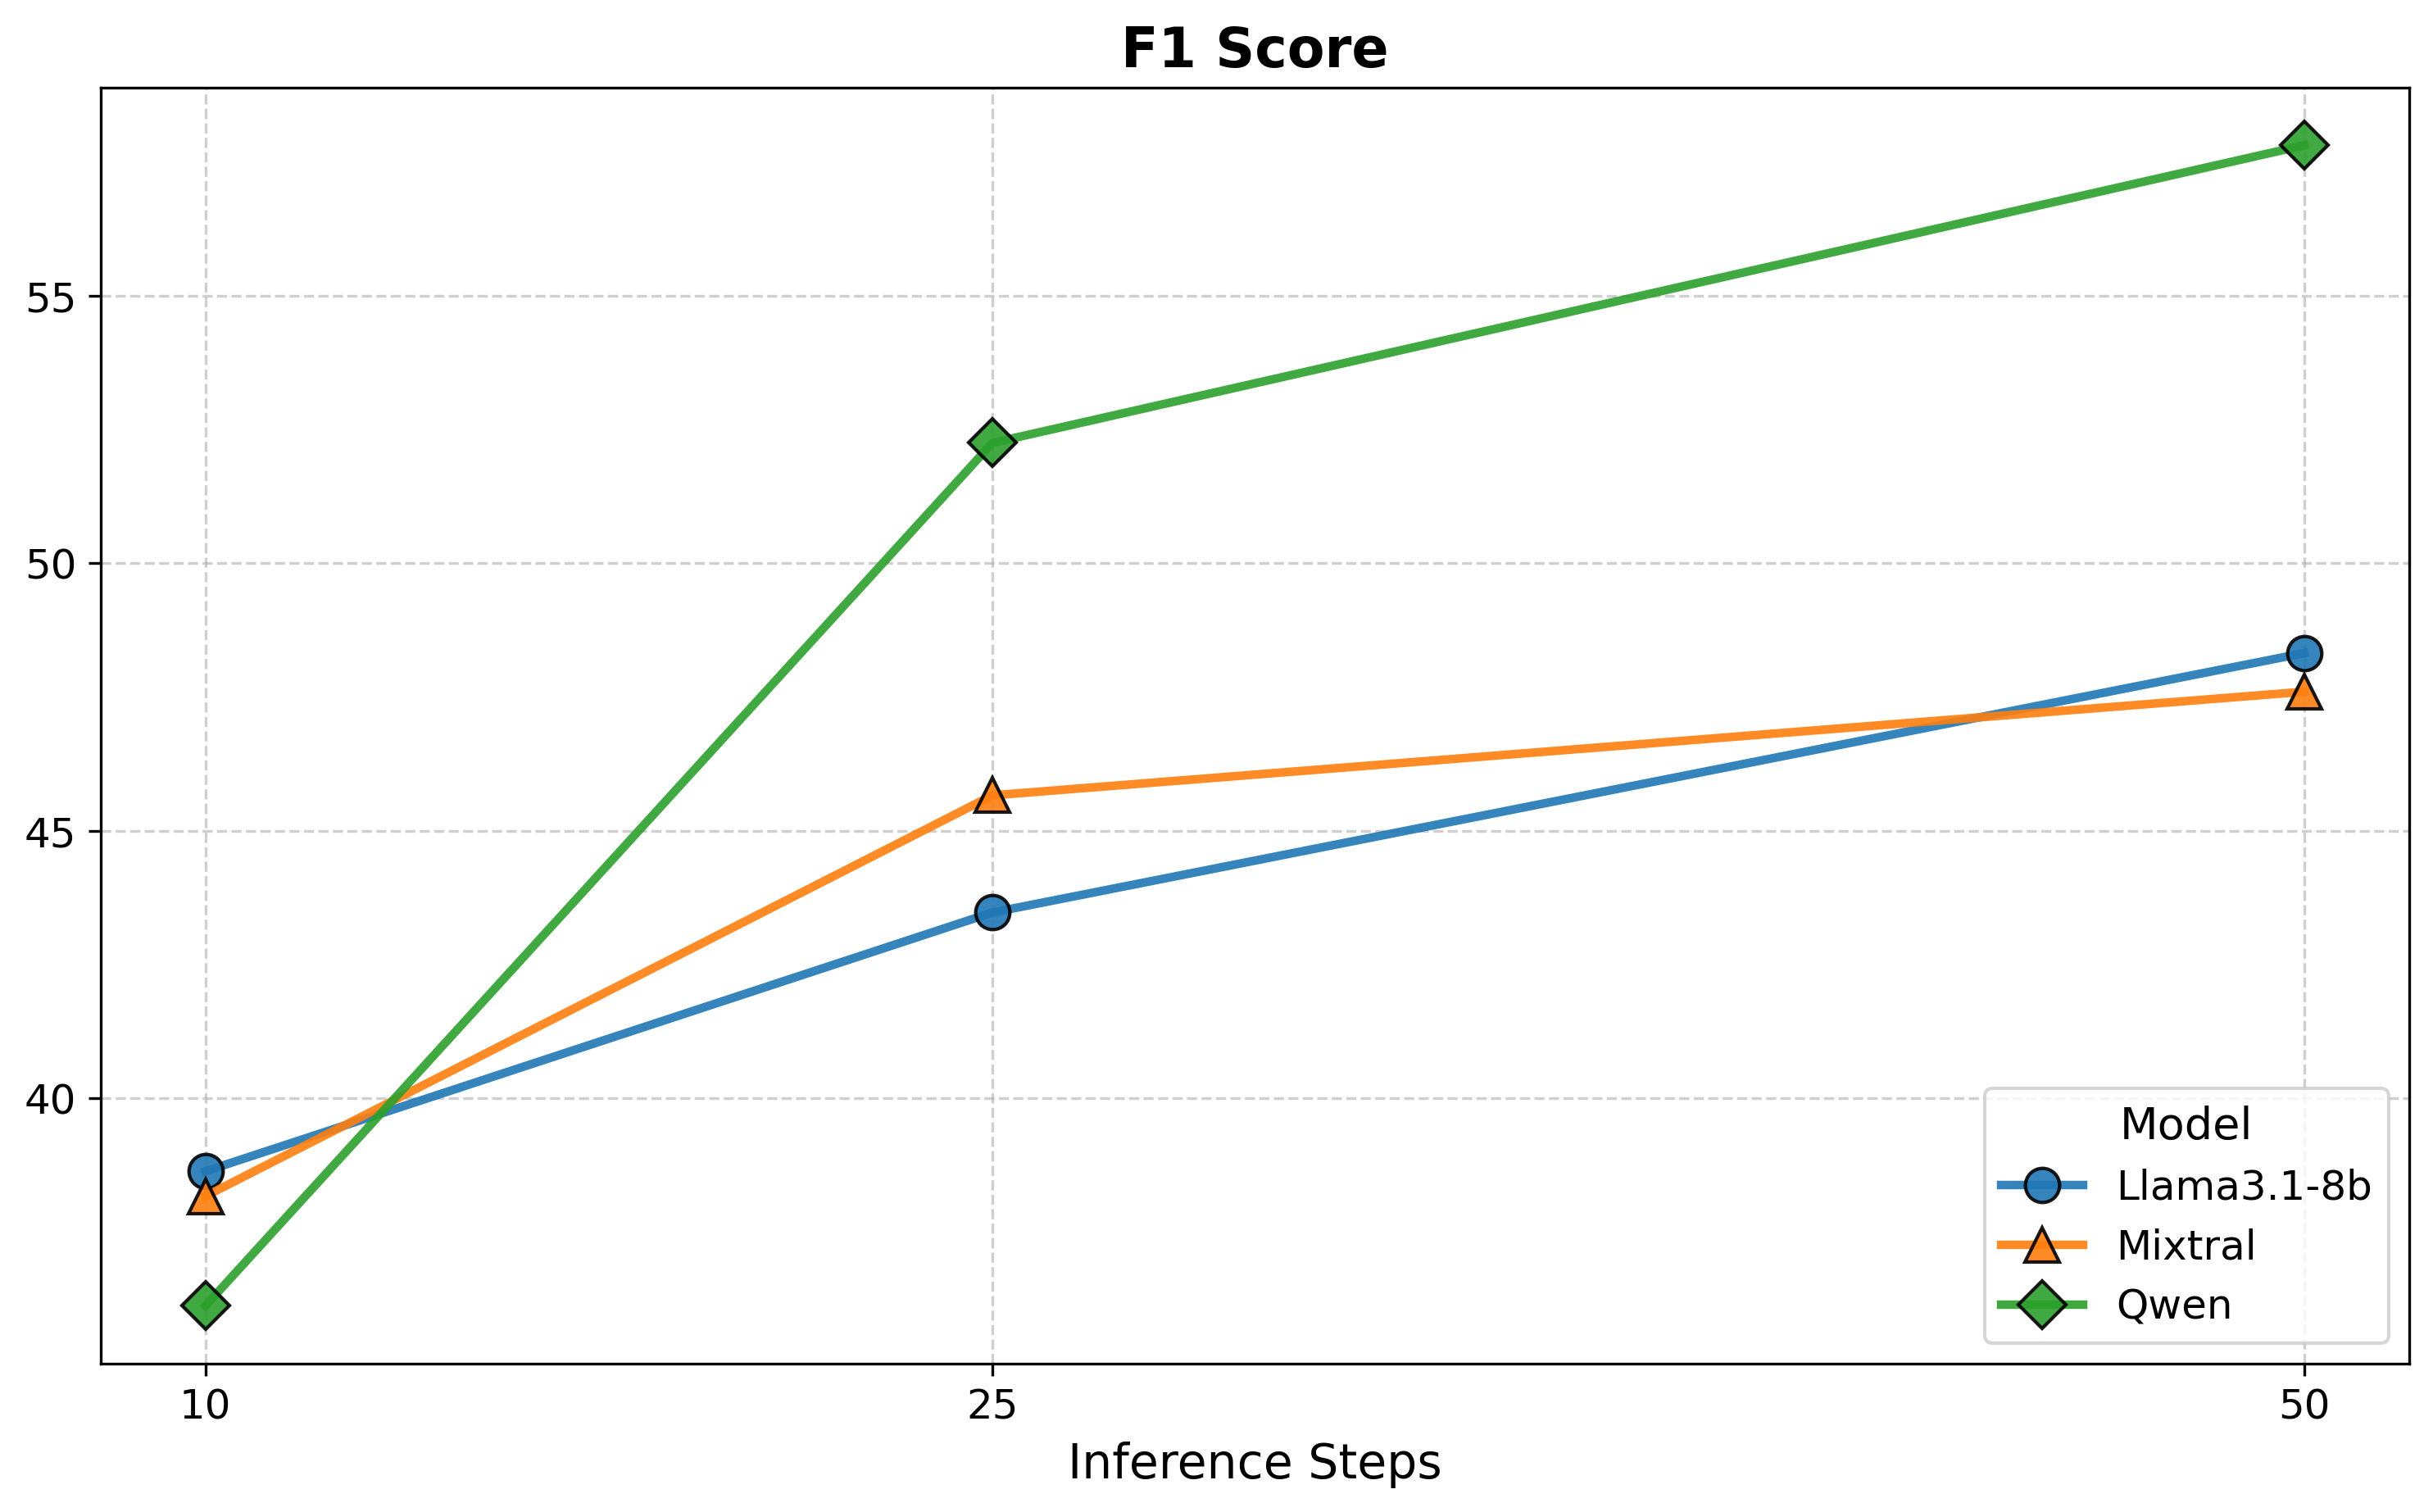
\includegraphics[width=\textwidth]{img/f1_score_majority_voting_1.png}
        \caption{F1 Scores}
        \label{fig:f1_scores}
    \end{subfigure}
    \hfill
    \begin{subfigure}[t]{0.48\textwidth}
        \centering
        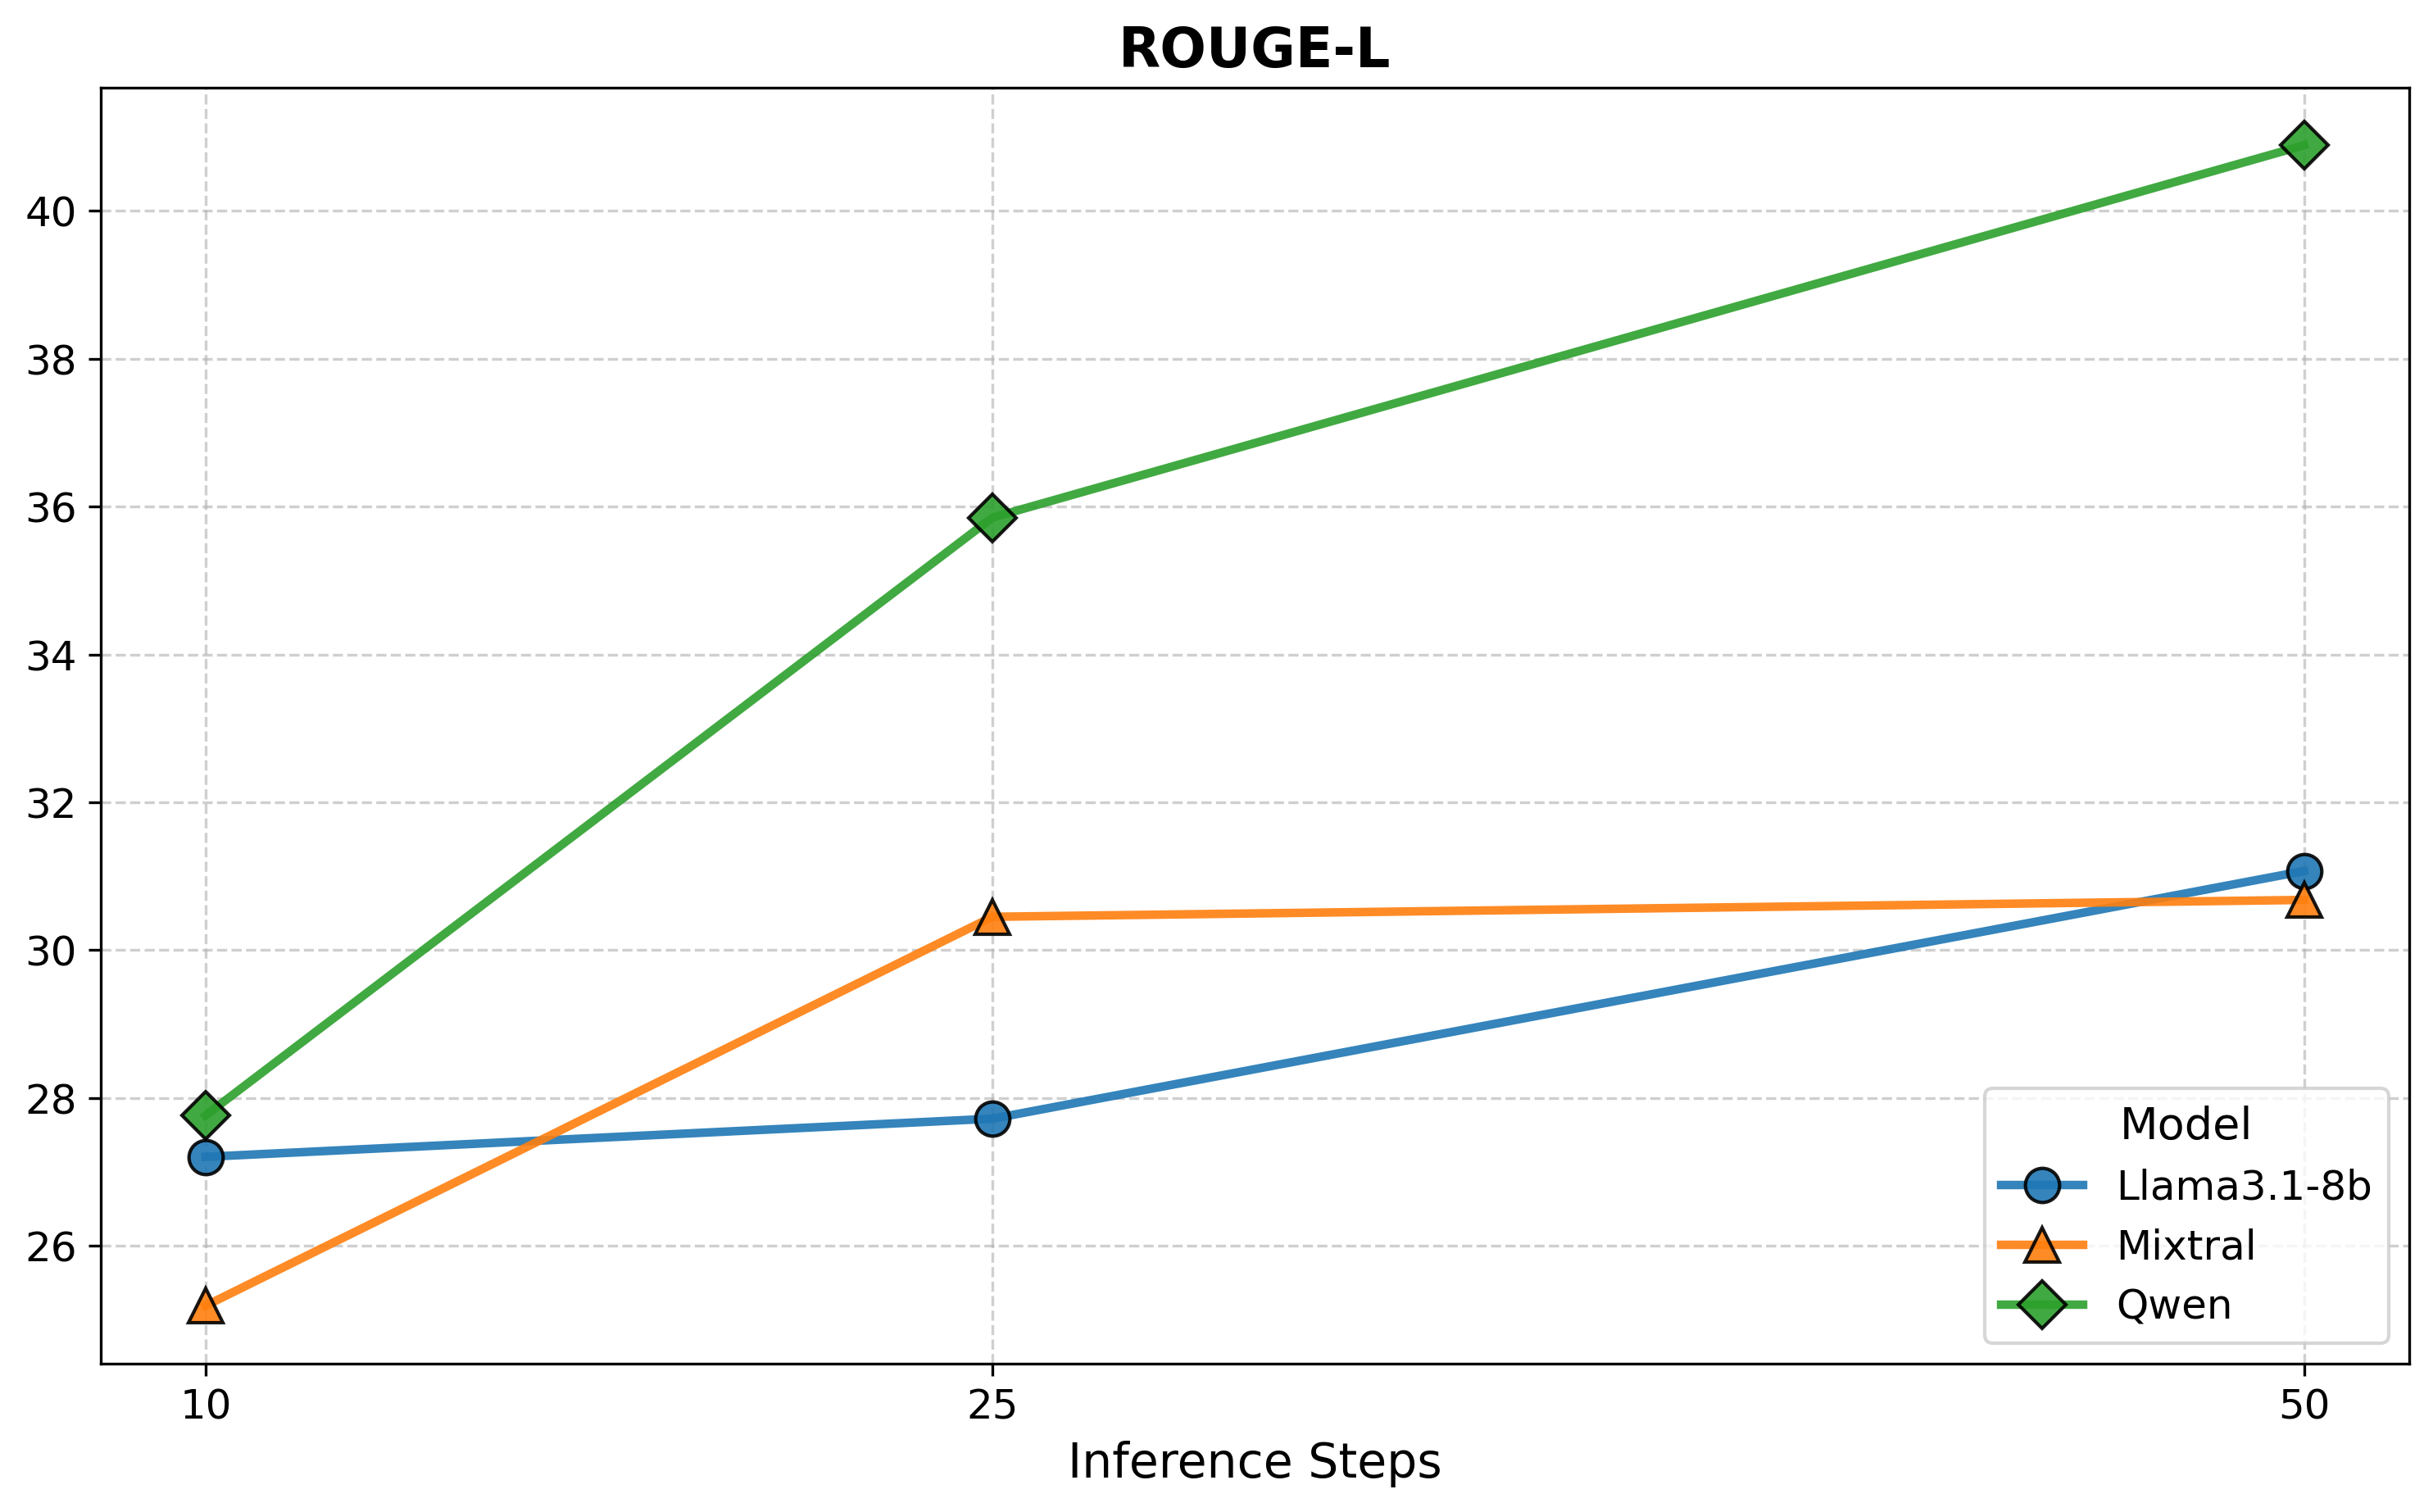
\includegraphics[width=\textwidth]{img/rougel_majority_voting_1.png}
        \caption{RougeL Scores}
        \label{fig:rougeL_scores}
    \end{subfigure}
    \caption{Performance of \textit{Inference Scaled GraphRAG} under varying inference step counts and model backbones including Llama3.1-8B-Instruct, Mixtral-8x7B-Instruct, and Qwen3-32b. 
    \textbf{(a)} F1 score increases consistently with more inference steps across all model configurations.  
    \textbf{(b)} RougeL scores show a similar trend, reflecting improvements in both symbolic and semantic alignment with ground-truth answers.}
    \label{fig:combined_scores}
\end{figure}